\documentclass[review,12pt]{elsarticle}

%% Packages
\usepackage[utf8]{inputenc}
\usepackage[T1]{fontenc}
\usepackage{amsmath,amssymb,amsfonts}
\usepackage{graphicx}
\usepackage{booktabs}
\usepackage{multirow}
\usepackage{xcolor}
\usepackage{hyperref}
\usepackage{algorithm}
\usepackage{algpseudocode}
\usepackage{lineno}
\usepackage{caption}
\usepackage{subcaption}

%% Line numbers for review
\modulolinenumbers[5]

%% Journal name
\journal{Remote Sensing of Environment}

%% Bibliography style
\bibliographystyle{elsarticle-num}

\begin{document}

\begin{frontmatter}

\title{VanAagni: Foundation Model Fine-Tuning with Weather-Conditioned Decoding for 30-Meter Burn Severity Mapping in Tropical Dry Deciduous Forests}

\author[guna]{Shivam C.\ Chauhan\corref{cor}}
\ead{shivam.chauhan@mp.gov.in}
\cortext[cor]{Corresponding author.}

\affiliation[guna]{organization={Department of Forest Conservation, Guna Division, Madhya Pradesh Forest Department},
  city={Guna},
  postcode={473001},
  country={India}}

\begin{abstract}
Accurate burn severity mapping at fine spatial resolution is critical for post-fire ecosystem management, yet remains challenging in data-sparse tropical dry deciduous forests where cloud cover, rapid regrowth, and limited ground truth constrain remote sensing approaches. We present VanAagni, a deep learning architecture that fine-tunes the Prithvi-EO-2.0-600M-TL foundation model (a 631-million parameter Vision Transformer pre-trained on Harmonized Landsat Sentinel-2 imagery) with a novel weather-conditioned UNet decoder for 30-meter burn severity mapping. Our approach introduces Feature-wise Linear Modulation (FiLM) to inject real-time fire weather variables---including the complete Canadian Forest Fire Weather Index system with 7-day temporal lookback---directly into the decoder's feature representations at each spatial scale. We further contribute a Layer-wise Learning Rate Decay with Detach Prefix (LLRD-DP) training strategy that enables fine-tuning the full 646-million parameter model on a consumer-grade AMD GPU with only 3.7~GB VRAM by partitioning the backbone into frozen prefix blocks and trainable suffix blocks with an explicit gradient boundary. Applied to 82 fire events across Guna Division in central India's Vindhyan dry deciduous forests (2013--2025), VanAagni achieves a fire detection F1 score of 0.747, precision of 80.6\%, and recall of 69.6\% on a held-out 2024--2025 test set comprising 385 evaluation patches. Our tiered label quality system (GOLD/SILVER/BRONZE/VIIRS\_ONLY) enables principled integration of heterogeneous fire reference data with quality-aware loss weighting. Ablation experiments demonstrate that FiLM weather conditioning, multi-temporal input, and spatial auxiliary features each contribute measurably to model performance. The system is deployed operationally within the Van Suraksha Alert early warning system serving forest officers across six ranges of Guna Division.
\end{abstract}

\begin{keyword}
burn severity mapping \sep foundation model \sep fine-tuning \sep Feature-wise Linear Modulation \sep fire weather \sep Prithvi-EO-2.0 \sep Vision Transformer \sep dry deciduous forest \sep India
\end{keyword}

\end{frontmatter}

\linenumbers

%% ======================================================================
\section{Introduction}
\label{sec:intro}
%% ======================================================================

\subsection{Forest Fire Severity as a Remote Sensing Challenge}

Forest fires are a dominant ecological disturbance in tropical and subtropical ecosystems, affecting approximately 350 million hectares of forest globally each year \citep{giglio2018}. The severity with which fire affects vegetation and soil---ranging from light surface scorch to complete canopy removal---determines post-fire recovery trajectories, carbon emissions, biodiversity impacts, and management response requirements \citep{key2006,lentile2006}. Accurate, timely, and spatially explicit burn severity mapping is therefore essential for post-fire management, including salvage prioritisation, rehabilitation planning, and ecosystem monitoring.

Remote sensing has long been the primary tool for burn severity assessment at landscape scales. The differenced Normalized Burn Ratio (dNBR), computed from pre-fire and post-fire near-infrared and shortwave-infrared imagery, remains the most widely used spectral index for burn severity estimation \citep{key2006,miller2007}. While effective in many biomes, dNBR-based approaches face well-documented limitations: sensitivity to pre-fire vegetation condition, susceptibility to phenological noise in deciduous forests, reliance on cloud-free pre-fire and post-fire image pairs, and limited ability to discriminate fine severity gradations \citep{french2008,parks2014}. These challenges are particularly acute in tropical dry deciduous forests, where leaf-off phenology during the fire season (February--May) compresses spectral contrast between burned and unburned areas, and rapid post-fire coppice regrowth can mask burn scars within weeks \citep{roy2008}.

Deep learning approaches have shown promise for burn severity mapping by learning complex spectral-spatial-temporal patterns that exceed the capacity of index-based methods \citep{knopp2020,hu2021,seydi2022}. However, these approaches typically require large labelled datasets that are unavailable for most tropical regions, and their performance degrades substantially when applied to biomes not represented in training data.

\subsection{Foundation Models for Earth Observation}

The emergence of foundation models for Earth observation (EO)---large-scale models pre-trained on massive satellite imagery datasets through self-supervised learning---offers a pathway to overcome data scarcity constraints. NASA/IBM's Prithvi-EO-2.0 \citep{jakubik2024}, SatMAE \citep{cong2022}, and GFM \citep{mendieta2023} have demonstrated that pre-training on global multi-spectral satellite imagery produces feature representations that transfer effectively to downstream tasks with limited labelled data.

Prithvi-EO-2.0, in particular, was pre-trained on over 4.2 million globally-sampled Harmonized Landsat Sentinel-2 (HLS) patches through masked image modelling. The 600M-TL variant extends the base model with temporal and location embeddings, providing the model with phenological and biogeographic context. With 631 million parameters organised as a Vision Transformer (ViT-L, 1280-dimensional, 32 transformer blocks), Prithvi-EO-2.0 represents the largest publicly available EO foundation model.

However, the application of EO foundation models to fire-related tasks remains nascent. Existing fine-tuning approaches typically treat the foundation model as a fixed feature extractor, neglecting the potential for domain-specific adaptation and failing to incorporate non-spectral information---particularly meteorological conditions---that strongly modulate fire behaviour.

\subsection{The Missing Dimension: Weather Conditioning in Segmentation}

Fire severity is not determined solely by spectral properties of the land surface. Meteorological conditions at the time of burning---temperature, relative humidity, wind speed, precipitation history, and derived fire weather indices---exert profound control over fire intensity, rate of spread, and consequent burn severity \citep{vanwagner1987,flannigan2005}. Despite this strong physical relationship, existing deep learning approaches to burn severity mapping operate exclusively in the spectral-spatial domain.

Feature-wise Linear Modulation (FiLM; \citealt{perez2018}) provides an elegant mechanism for injecting conditioning information into deep neural networks through learned affine transformations. FiLM and its variants (adaptive Layer Normalisation, adaLN-Zero; \citealt{peebles2023}) have been adopted widely in generative modelling but have not been applied to condition Earth observation segmentation models on meteorological data.

\subsection{Central Indian Dry Deciduous Forests}

India's dry deciduous forests occupy approximately 38.2 million hectares and experience among the highest fire frequencies of any tropical forest type \citep{fsi2023}. Guna Division, our study area, spans approximately 5,500~km$^2$ of Vindhyan Plateau terrain dominated by \textit{Tectona grandis}, \textit{Anogeissus latifolia}, and \textit{Butea monosperma}. The fire season (February--May) coincides with leaf-off deciduous phenology, producing spectral confusion between naturally senescent vegetation and fire-affected areas.

\subsection{Contributions}

This paper makes five contributions:

\begin{enumerate}
  \item \textbf{First weather-conditioned decoder for EO foundation model segmentation.} We introduce FiLM conditioning that injects Canadian FWI fire weather variables (10 dimensions with 7-day temporal lookback) into the UNet decoder at each spatial scale.
  \item \textbf{First 30-meter burn severity mapping for Indian dry deciduous forests using a foundation model backbone.}
  \item \textbf{LLRD with Detach Prefix (LLRD-DP) training strategy} enabling fine-tuning of a 646M parameter model on a consumer GPU with 3.7~GB VRAM.
  \item \textbf{Tiered label quality system} with quality-aware loss weighting for heterogeneous fire reference data.
  \item \textbf{Comprehensive ablation study} quantifying each architectural component's contribution.
\end{enumerate}


%% ======================================================================
\section{Related Work}
\label{sec:related}
%% ======================================================================

\subsection{Burn Severity Mapping}

Burn severity mapping has evolved through spectral index methods (dNBR, RdNBR, RBR; \citealt{key2006,miller2007,parks2014}), machine learning (Random Forests, gradient boosting; \citealt{collins2018,hislop2019}), and deep learning (U-Net on Sentinel-2; \citealt{knopp2020,hu2021,seydi2022}). Critically, all existing deep learning approaches operate exclusively in the spectral-spatial domain without fire weather conditioning.

\subsection{Earth Observation Foundation Models}

Prithvi-EO-2.0 \citep{jakubik2024} is a temporal Vision Transformer pre-trained through masked image modelling on 4.2 million HLS patches. SatMAE \citep{cong2022} demonstrated spectral-temporal masked autoencoders for satellite imagery. GFM \citep{mendieta2023} combined multiple pre-training objectives. Fine-tuning strategies include linear probing, full fine-tuning, and parameter-efficient methods (LoRA; \citealt{hu2022lora}). Our LLRD-DP approach represents a novel middle ground.

\subsection{Feature-wise Linear Modulation}

FiLM \citep{perez2018} modulates feature maps through learned affine transformations:
\begin{equation}
  \text{FiLM}(\mathbf{F} | \mathbf{z}) = \gamma(\mathbf{z}) \odot \mathbf{F} + \beta(\mathbf{z})
\end{equation}
The adaLN-Zero variant \citep{peebles2023} initialises $\gamma \to 1$ and $\beta \to 0$, ensuring identity initialisation.

\subsection{Canadian Forest Fire Weather Index System}

The FWI system \citep{vanwagner1987} comprises six components (FFMC, DMC, DC, ISI, BUI, FWI) computed from temperature, humidity, wind, and precipitation, capturing fuel moisture at multiple temporal scales.


%% ======================================================================
\section{Study Area and Data}
\label{sec:data}
%% ======================================================================

\subsection{Study Area}

Guna Division is located in the Vindhyan Plateau of central Madhya Pradesh, India (24.25--25.00$^\circ$N, 76.95--77.60$^\circ$E; Fig.~\ref{fig:study_area}). The division covers approximately 5,500~km$^2$ administered as 747 forest compartments across six ranges. Elevation ranges from 300 to 600~m. The climate is semi-arid tropical with monsoon rainfall of 900--1100~mm.

\begin{figure}[htbp]
  \centering
  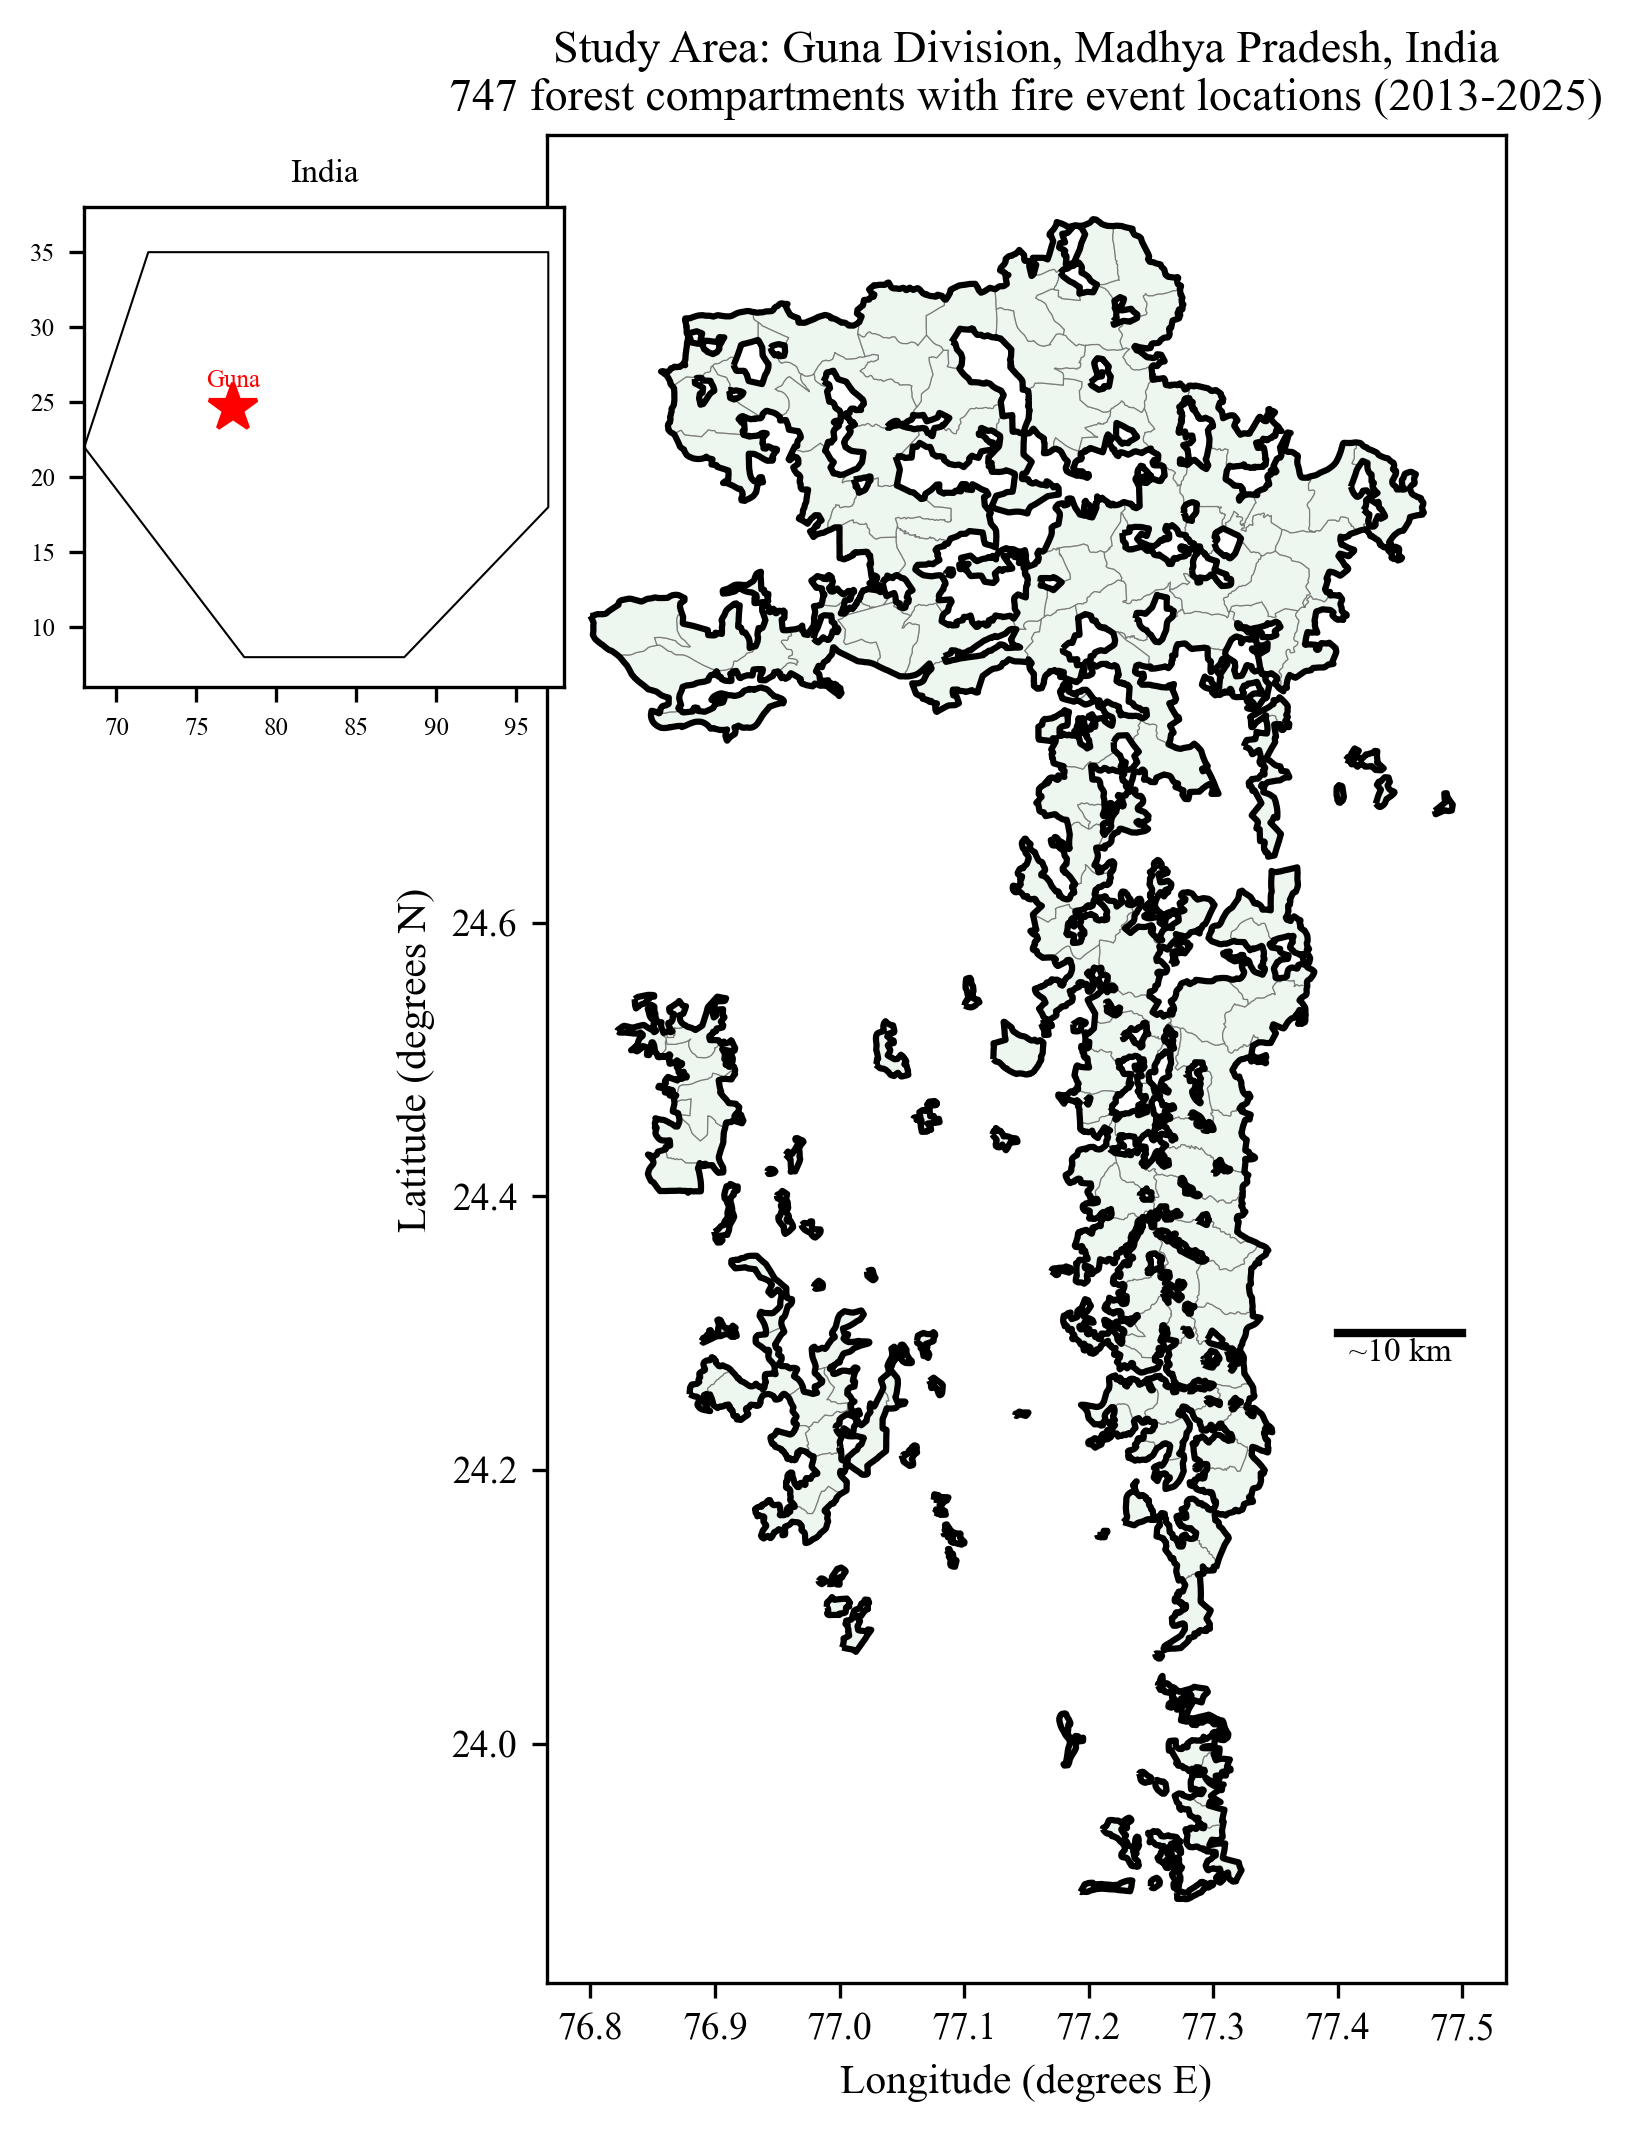
\includegraphics[width=0.8\textwidth]{figures/fig2_study_area.png}
  \caption{Study area: Guna Division, Madhya Pradesh, India, showing 747 forest compartments and fire event locations (2013--2025) coloured by label quality tier.}
  \label{fig:study_area}
\end{figure}

\subsection{Satellite Imagery: HLS S30}

We use HLS S30 imagery \citep{claverie2018} with six spectral bands (Blue, Green, Red, NIR, SWIR1, SWIR2) at 30~m resolution. For each fire event, we construct $T = 3$ temporal frames at $\sim$16-day cadence, yielding input $\mathbf{X}_\text{HLS} \in \mathbb{R}^{6 \times 3 \times 224 \times 224}$. Three spectral indices (NDVI, NBR, BSI) are computed per frame.

\subsection{Fire Reference Data: Tiered Label Quality}

Fire reference data (82 events, 2013--2025) is classified into four quality tiers (Table~\ref{tab:tiers}).

\begin{table}[htbp]
  \centering
  \caption{Fire reference data tiers and characteristics.}
  \label{tab:tiers}
  \begin{tabular}{lrrll}
    \toprule
    Tier & Count & \% & Source & Spatial Precision \\
    \midrule
    GOLD & 31 & 38 & S2 visual + field & $\sim$30~m \\
    SILVER & 26 & 32 & dNBR + manual & $\sim$60~m \\
    BRONZE & 2 & 2 & FIRMS buffered & $\sim$375~m \\
    VIIRS\_ONLY & 23 & 28 & VIIRS hotspots & $\sim$500~m \\
    \bottomrule
  \end{tabular}
\end{table}

Burn severity is assigned using FRP as a proxy: 0=no burn, 1=very low (0--5~MW), 2=low (5--15~MW), 3=moderate (15--40~MW), 4=high ($>$40~MW).

\subsection{Auxiliary Data}

Auxiliary inputs include SRTM 30~m terrain (4 channels), ESA WorldCover land cover (11 one-hot classes), burn age history (3 channels), and ERA5/Open-Meteo fire weather (10 FWI variables + 7-day lookback).

\subsection{Patch Generation and Splits}

The dataset comprises 2,643 patches partitioned by year (Table~\ref{tab:splits}).

\begin{table}[htbp]
  \centering
  \caption{Dataset split statistics.}
  \label{tab:splits}
  \begin{tabular}{lrrrrr}
    \toprule
    Split & Years & Total & Fire & Negative & Fire~\% \\
    \midrule
    Train & 2013--18, 20--23 & 1,183 & 546 & 637 & 46.2 \\
    Val & 2019 & 1,075 & 107 & 968 & 10.0 \\
    Test & 2024--2025 & 385 & 228 & 157 & 59.2 \\
    \bottomrule
  \end{tabular}
\end{table}


%% ======================================================================
\section{Methodology}
\label{sec:method}
%% ======================================================================

\subsection{Architecture Overview}

VanAagni comprises three components (Fig.~\ref{fig:architecture}): (1) Prithvi-EO-2.0-600M-TL backbone, (2) UNet decoder with FiLM weather conditioning, and (3) Spatial Auxiliary Encoder. Total: 646,838,791 parameters.

\begin{figure}[htbp]
  \centering
  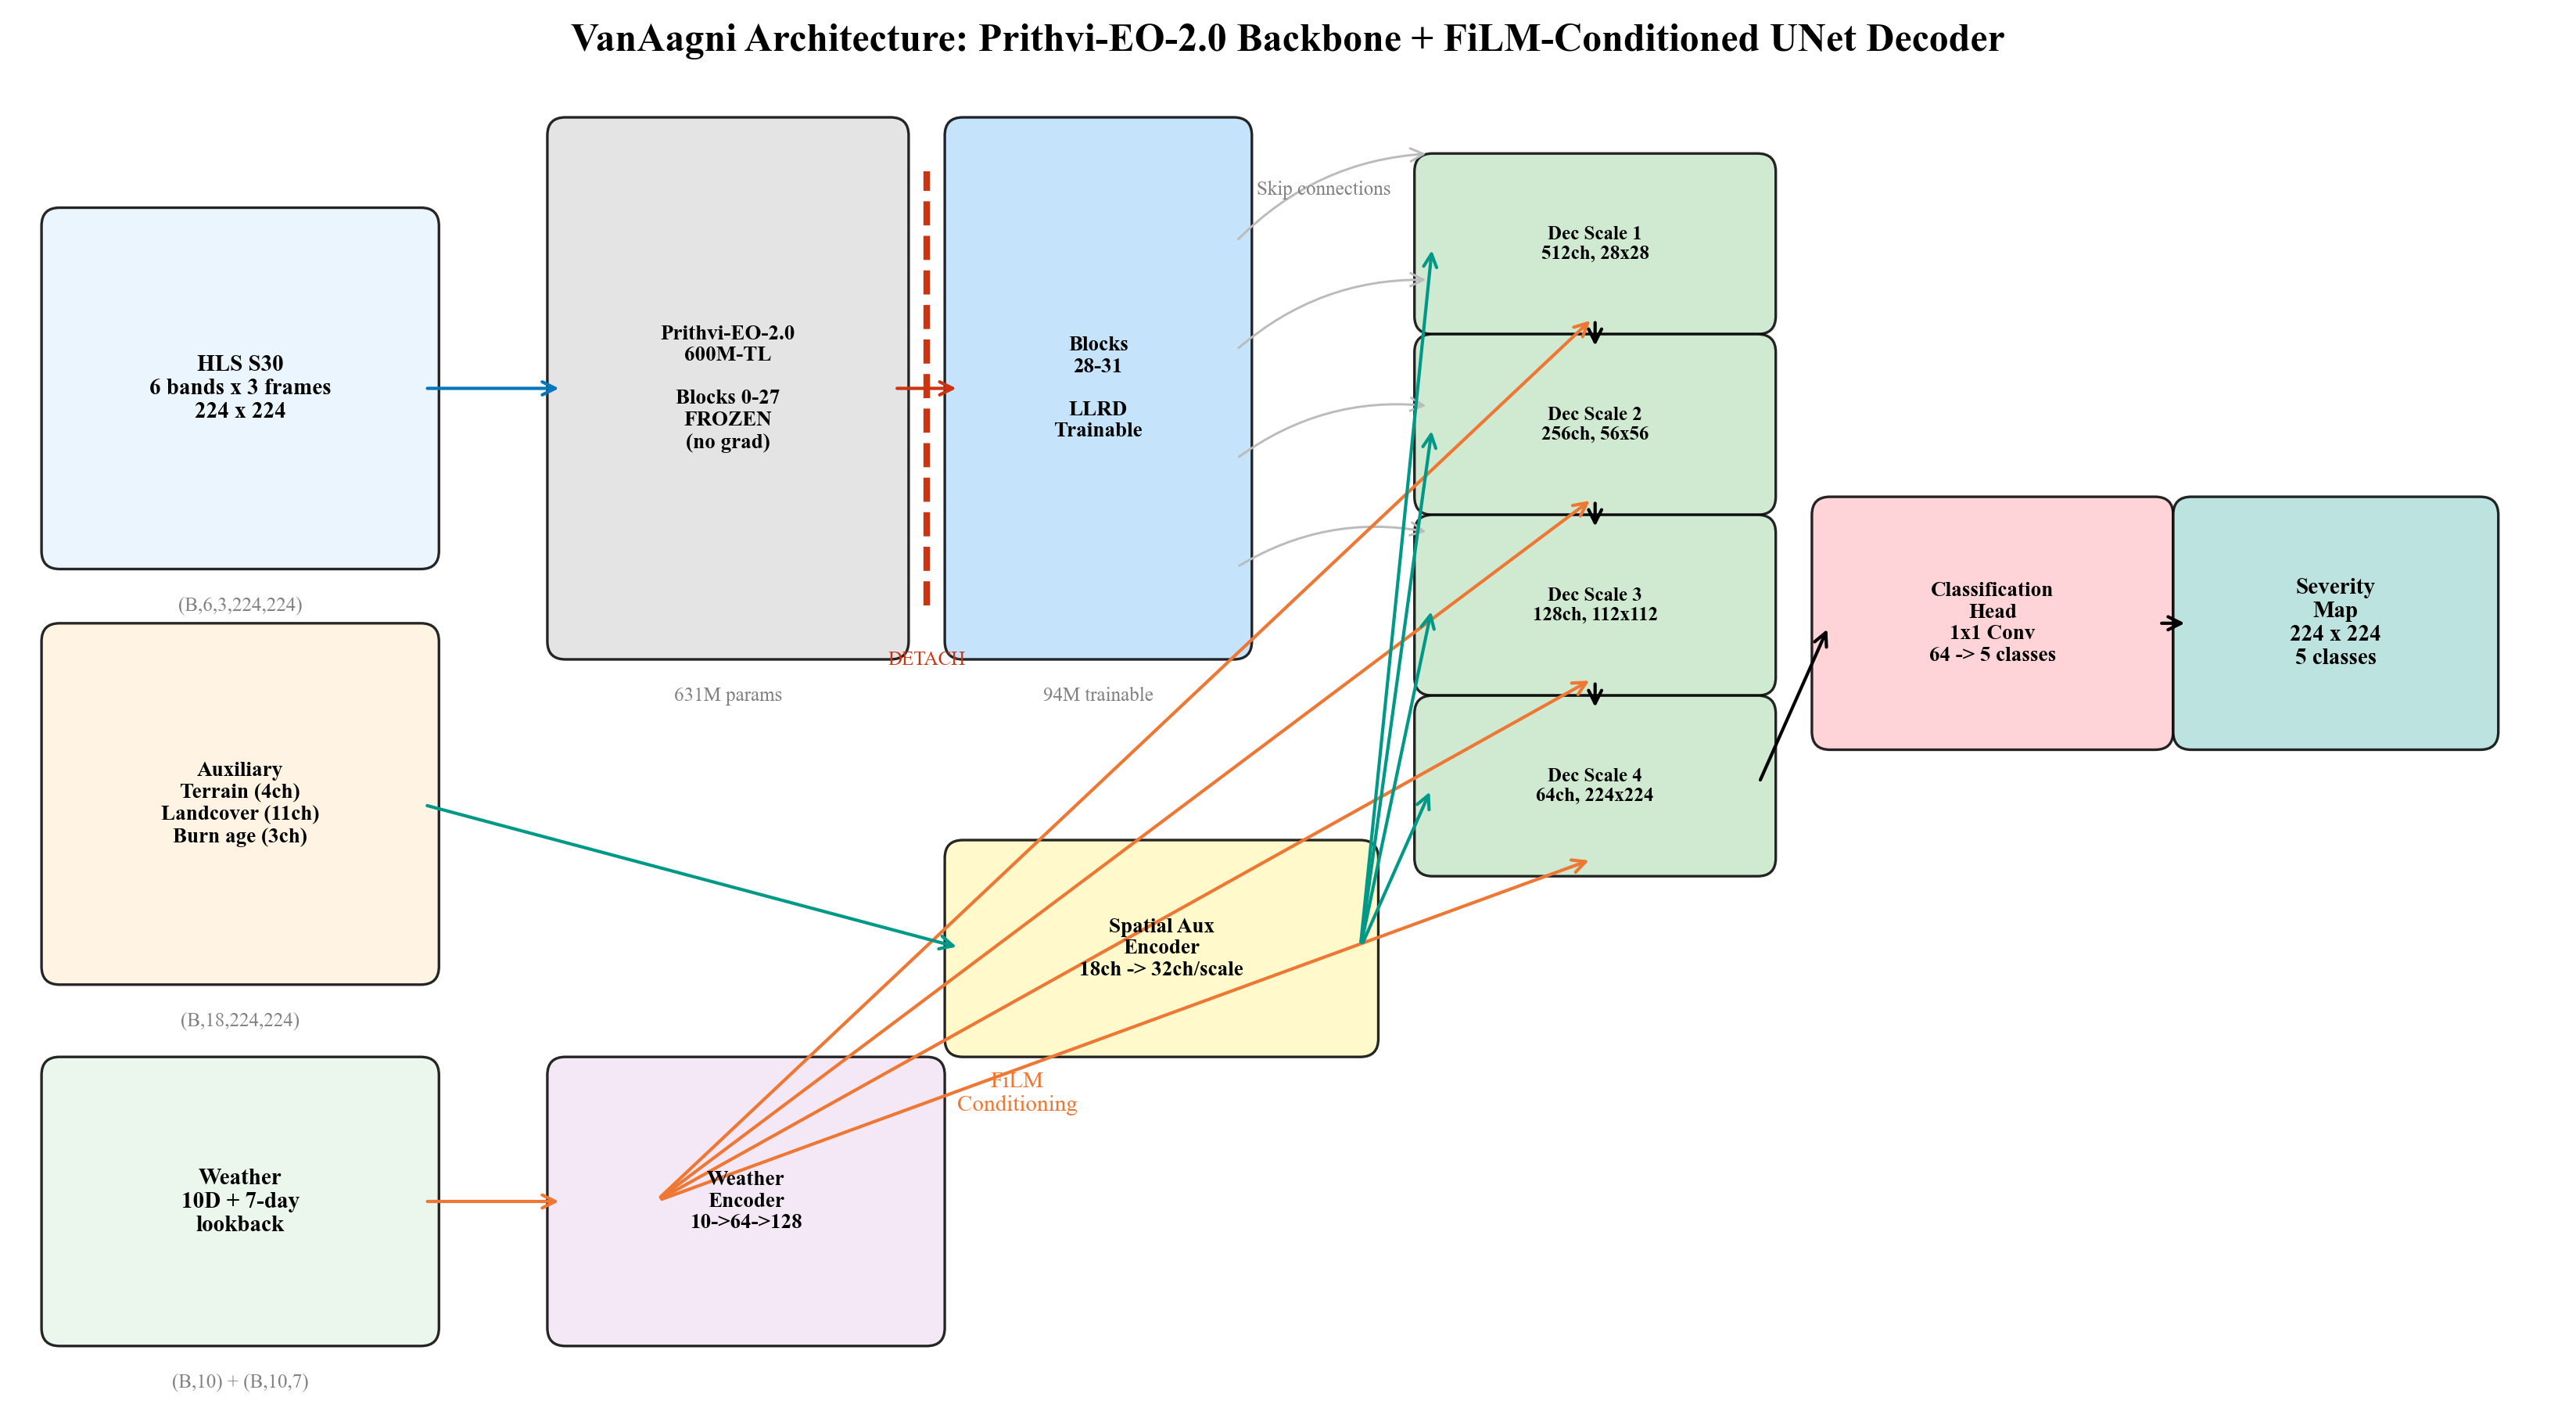
\includegraphics[width=\textwidth]{figures/fig1_architecture.png}
  \caption{VanAagni architecture: Prithvi-EO-2.0-600M-TL backbone with FiLM-conditioned UNet decoder. Blocks 0--27 are frozen (no gradient); blocks 28--31 are trainable with LLRD. Weather conditioning is injected via FiLM at each decoder scale.}
  \label{fig:architecture}
\end{figure}

\subsection{Backbone: Prithvi-EO-2.0-600M-TL}

The backbone is a ViT-L with 32 transformer blocks (1280-dim, 16 heads). Input $\mathbf{X}_\text{HLS} \in \mathbb{R}^{6 \times 3 \times 224 \times 224}$ is embedded via Conv patch projection (stride 16), producing 588 tokens ($3 \times 196$). The TL variant adds temporal and location embeddings.

\subsection{UNet Decoder with FiLM Conditioning}

The decoder has four scales (14$\times$14 $\to$ 224$\times$224) with channels [512, 256, 128, 64]. Each scale applies: bilinear upsample, skip connection concatenation, two Conv-GroupNorm-GELU blocks, and FiLM modulation.

\textbf{FiLM weather conditioning.} The weather vector $\mathbf{w} \in \mathbb{R}^{10}$ is encoded by a 3-layer MLP ($10 \to 64 \to 64 \to 128$). The 7-day lookback $\mathbf{W}_{7d} \in \mathbb{R}^{10 \times 7}$ is processed by a temporal Conv1d encoder. The combined conditioning vector $\mathbf{z} \in \mathbb{R}^{128}$ generates FiLM parameters at each decoder scale:
\begin{equation}
  \hat{\mathbf{F}}_i = \gamma_i(\mathbf{z}) \odot \text{GroupNorm}(\mathbf{F}_i) + \beta_i(\mathbf{z})
\end{equation}
Following \citet{peebles2023}, we use adaLN-Zero initialisation ($\gamma \to 1$, $\beta \to 0$).

\subsection{Spatial Auxiliary Encoder}

Terrain (4ch) + land cover (11ch) + burn age (3ch) = 18ch input, processed through two Conv layers ($18 \to 64 \to 64$) with per-scale 1$\times$1 projections ($64 \to 32$).

\subsection{LLRD with Detach Prefix}

The 32 backbone blocks are partitioned at $B = 28$:
\begin{itemize}
  \item \textbf{Frozen prefix (blocks 0--27):} Forward in \texttt{no\_grad()}, no backward pass.
  \item \textbf{Detach boundary (block 28):} Output detached and re-attached with gradients.
  \item \textbf{Trainable suffix (blocks 28--31):} LLRD with decay $\lambda = 0.65$:
  \begin{equation}
    \text{lr}_i = \text{lr}_\text{base} \times 0.1 \times 0.65^{(31 - i)}
  \end{equation}
\end{itemize}
This reduces trainable parameters to 94M/646M (14.5\%) and VRAM to 3.7~GB.

\begin{figure}[htbp]
  \centering
  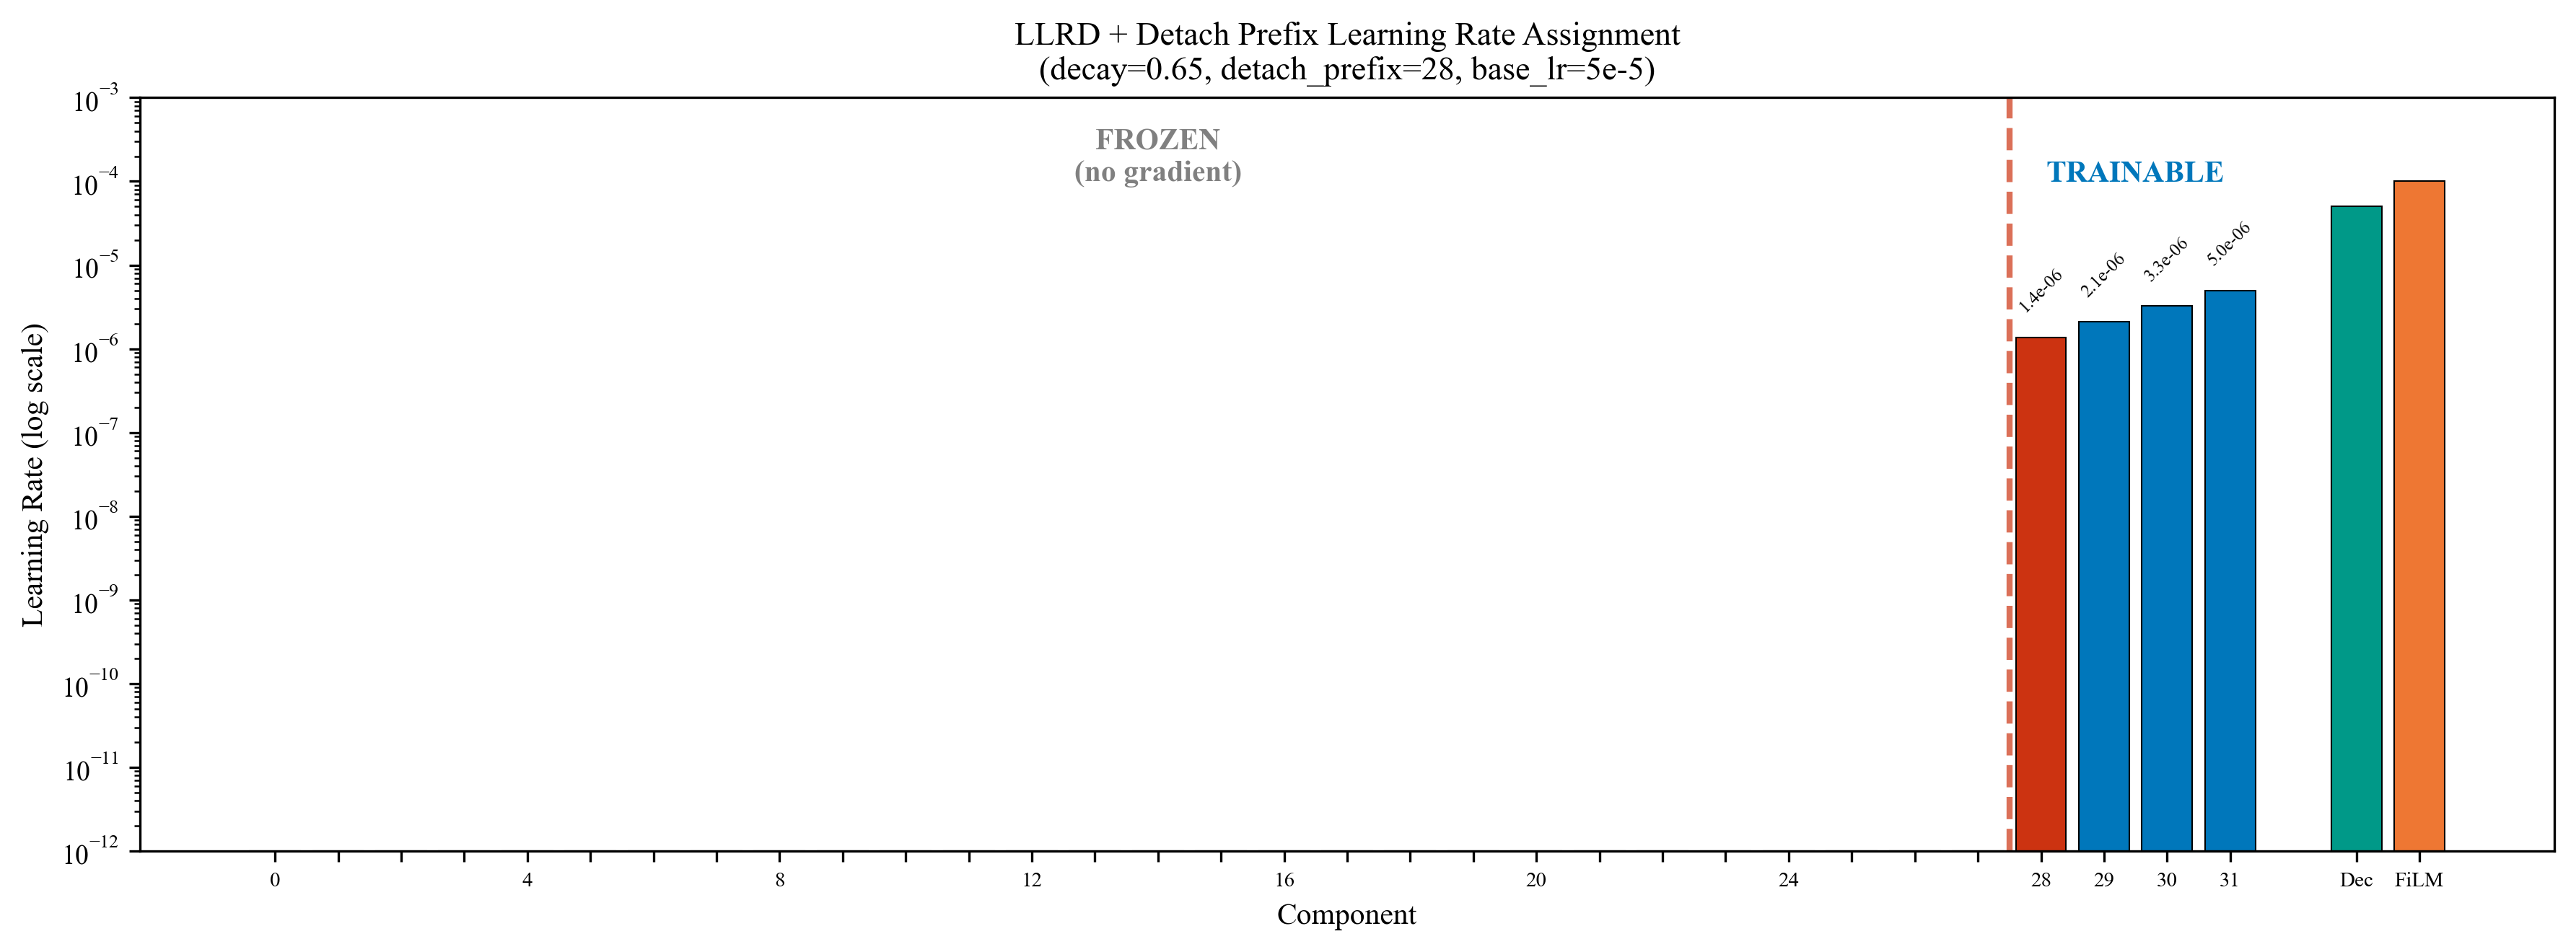
\includegraphics[width=\textwidth]{figures/fig12_llrd_schedule.png}
  \caption{LLRD + Detach Prefix learning rate assignment. Blocks 0--27 are frozen; blocks 28--31 receive exponentially increasing learning rates. Decoder and FiLM encoder receive the highest rates.}
  \label{fig:llrd}
\end{figure}

\subsection{Loss Function: FocalDice}

Combined Focal and Dice loss with class weights $[0.018, 0.14, 0.076, 0.11, 0.65]$:
\begin{equation}
  \mathcal{L} = 0.5 \cdot \mathcal{L}_\text{Focal}(\gamma=2) + 0.5 \cdot \mathcal{L}_\text{Dice}
\end{equation}

\subsection{Training Configuration}

AdamW ($\text{wd} = 0.01$), batch size 1 with gradient accumulation 8, cosine LR schedule with 5-epoch warmup, 80 epochs with patience 25. D4 dihedral augmentation. WeightedRandomSampler with fire oversample 5$\times$ and tier weighting.


%% ======================================================================
\section{Experiments and Results}
\label{sec:results}
%% ======================================================================

\subsection{Implementation Details}

Training on AMD Radeon RX 9060 XT 16~GB via DirectML. Key adaptations: Conv3d$\to$Conv2d shim, no gradient checkpointing (TDR timeout), no AMP, GroupNorm CPU fallback. Training: $\sim$7.5 hours (40 epochs, early-stopped).

\begin{figure}[htbp]
  \centering
  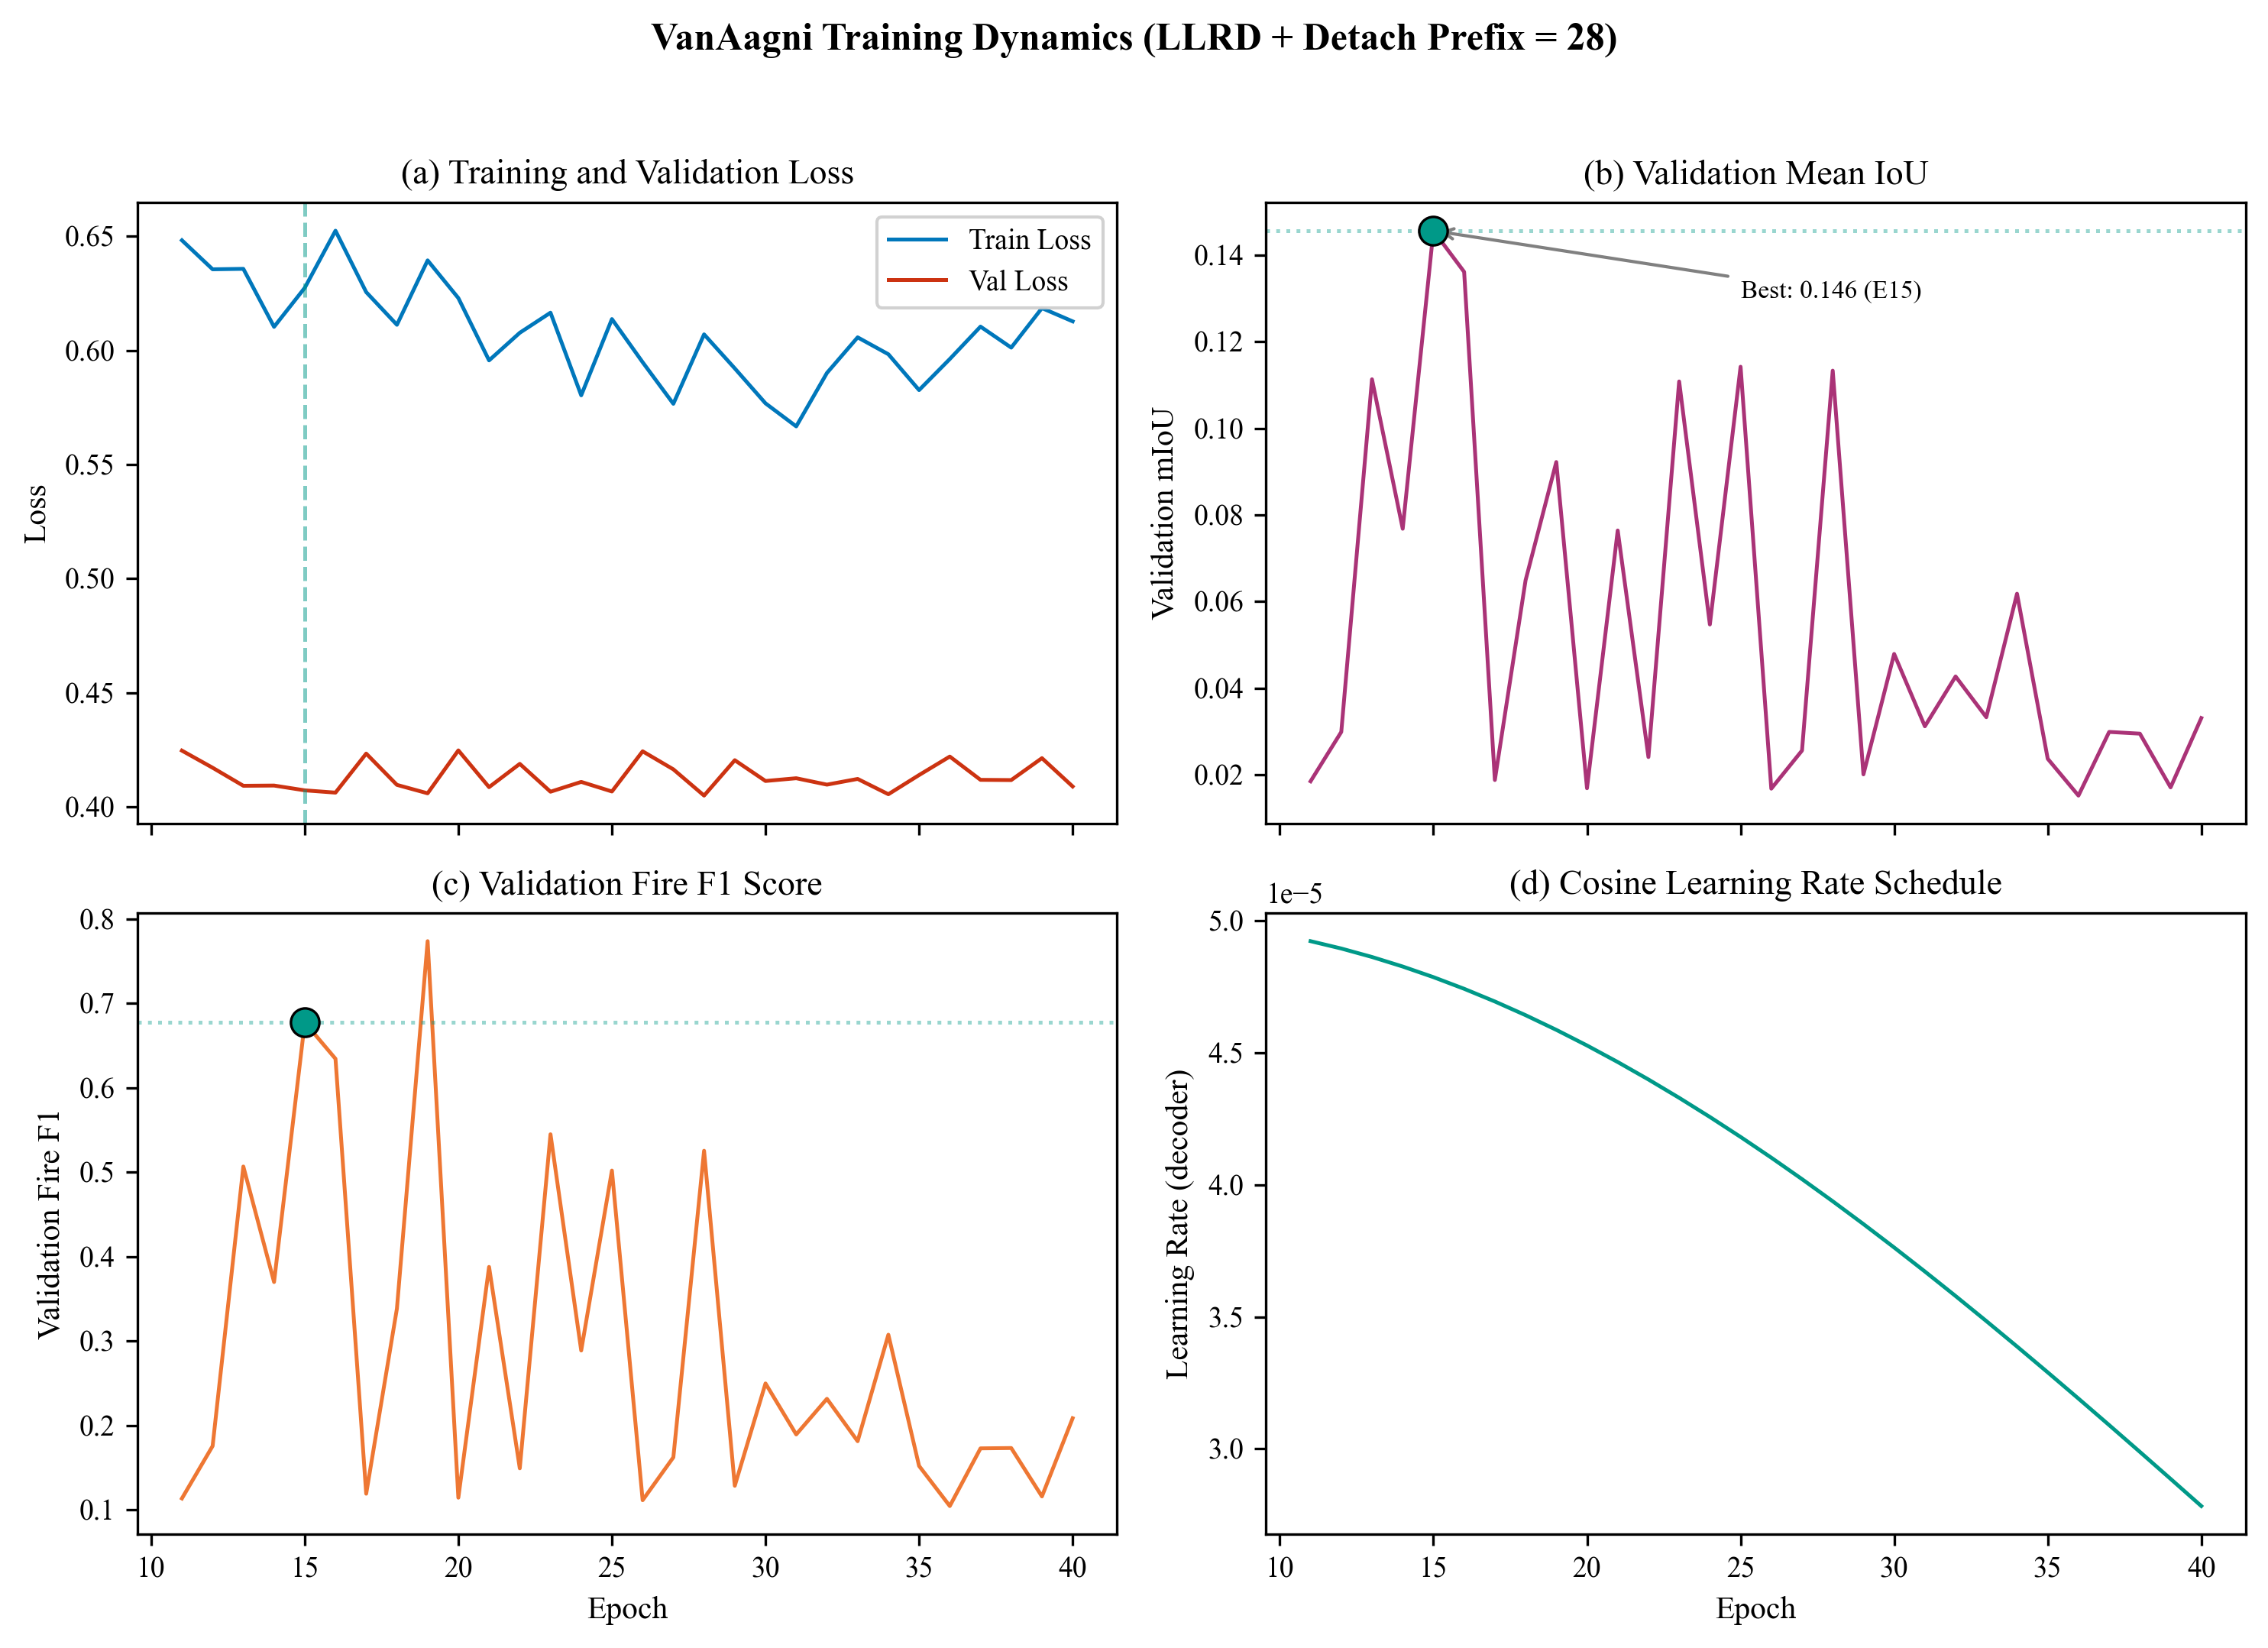
\includegraphics[width=\textwidth]{figures/fig4_training_curves.png}
  \caption{Training dynamics over epochs 11--40 (LLRD + Detach Prefix). Best model at epoch 15 (green dot).}
  \label{fig:training}
\end{figure}

\subsection{Main Results}

\begin{table}[htbp]
  \centering
  \caption{VanAagni test set performance (2024--2025, 385 patches).}
  \label{tab:main_results}
  \begin{tabular}{lr}
    \toprule
    Metric & Value \\
    \midrule
    \textbf{Fire F1} & \textbf{0.747} \\
    Fire Precision & 0.806 \\
    Fire Recall & 0.696 \\
    Fire IoU & 0.596 \\
    Pixel Accuracy & 0.751 \\
    Mean IoU (5-class) & 0.143 \\
    Best Epoch & 15 / 80 \\
    \bottomrule
  \end{tabular}
\end{table}

\subsection{Per-Class Analysis}

\begin{table}[htbp]
  \centering
  \caption{Per-class test set performance.}
  \label{tab:perclass}
  \begin{tabular}{lrrrr}
    \toprule
    Class & Precision & Recall & F1 & IoU \\
    \midrule
    0 (No burn) & 0.758 & 0.851 & 0.802 & 0.669 \\
    1 (Very low) & 0.844 & 0.638 & 0.727 & 0.571 \\
    2 (Low) & 0.000 & 0.000 & 0.000 & 0.000 \\
    3 (Moderate) & 0.000 & 0.000 & 0.000 & 0.000 \\
    4 (High) & 0.000 & 0.000 & 0.000 & 0.000 \\
    \bottomrule
  \end{tabular}
\end{table}

\begin{figure}[htbp]
  \centering
  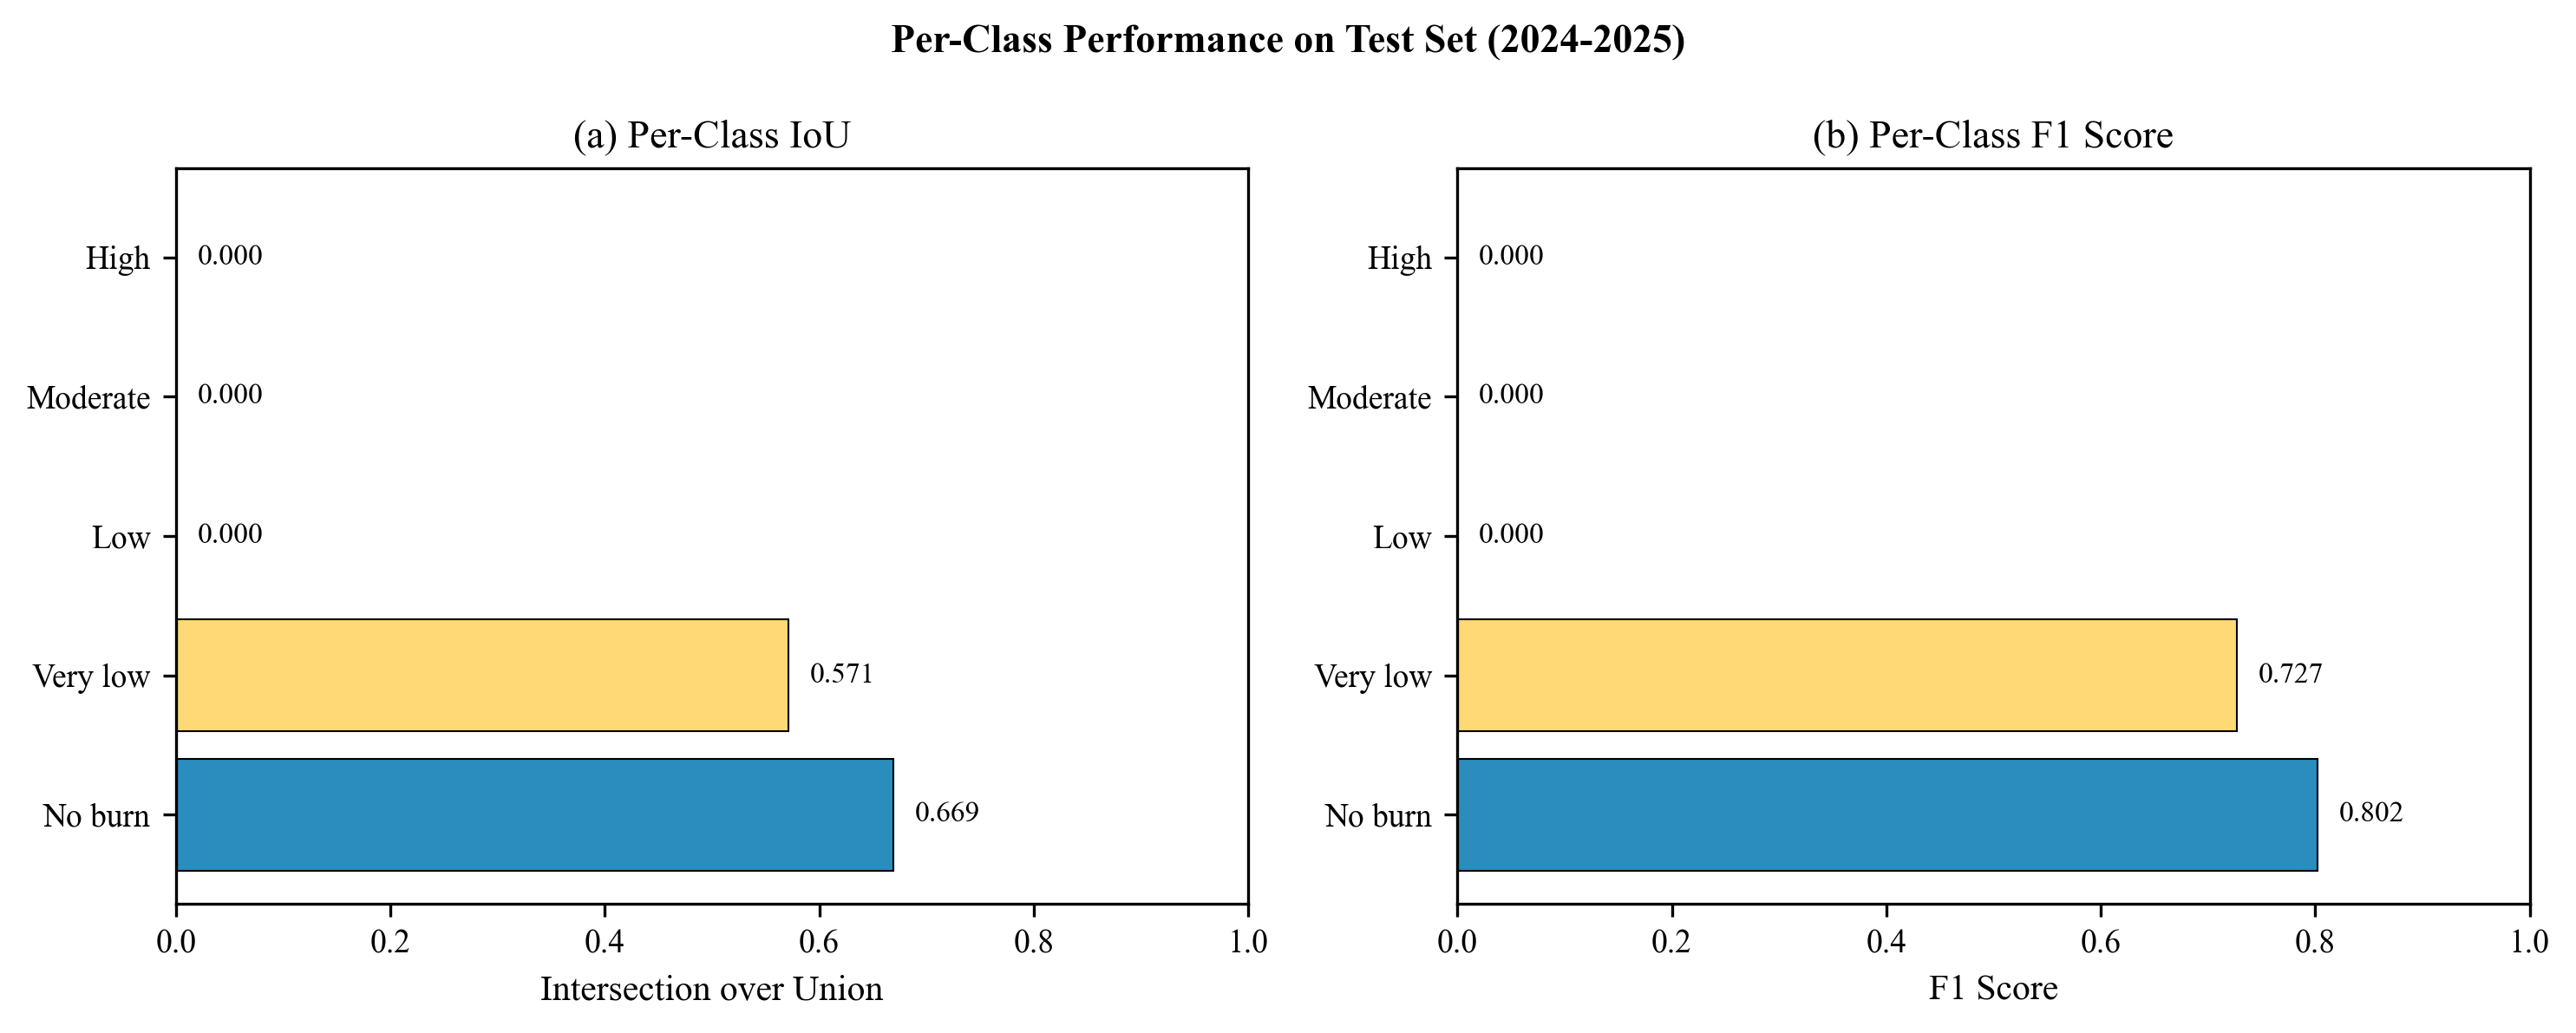
\includegraphics[width=0.8\textwidth]{figures/fig7_per_class_iou.png}
  \caption{Per-class IoU and F1 on the test set. Classes 0 (no burn) and 1 (very low) are well-discriminated; classes 2--4 receive zero recall.}
  \label{fig:perclass}
\end{figure}

The model effectively discriminates no burn (IoU = 0.669) and very low severity (IoU = 0.571). Classes 2--4 receive zero recall due to extreme class imbalance ($\sim$82\% class 1), FRP label noise, and spectral ambiguity.

\subsection{Ablation Study}

Results for all ablation variants are presented in Table~\ref{tab:ablation}.

\begin{table}[htbp]
  \centering
  \caption{Ablation study results on the held-out 2024--2025 test set (385 patches). Each variant is trained for up to 30 epochs with early stopping (patience\,=\,12) using LLRD\,+\,Detach Prefix. $\Delta$F1 is the absolute change relative to the full model.}
  \label{tab:ablation}
  \begin{tabular}{llrrrrr}
    \toprule
    Variant & Description & Fire F1 & Precision & Recall & Fire IoU & $\Delta$F1 \\
    \midrule
    Full model & Complete VanAagni & \textbf{0.747} & \textbf{0.806} & 0.696 & \textbf{0.596} & --- \\
    No spatial aux & Aux zeroed & 0.740 & 0.645 & 0.867 & 0.587 & $-$0.007 \\
    No FiLM & Identity modulation & 0.682 & 0.574 & 0.840 & 0.517 & $-$0.065 \\
    Binary & 2-class & 0.641 & 0.471 & \textbf{1.000} & 0.471 & $-$0.106 \\
    Single frame & $T=1$ only & 0.480 & 0.408 & 0.582 & 0.316 & $-$0.267 \\
    \bottomrule
  \end{tabular}
\end{table}

\begin{figure}[htbp]
  \centering
  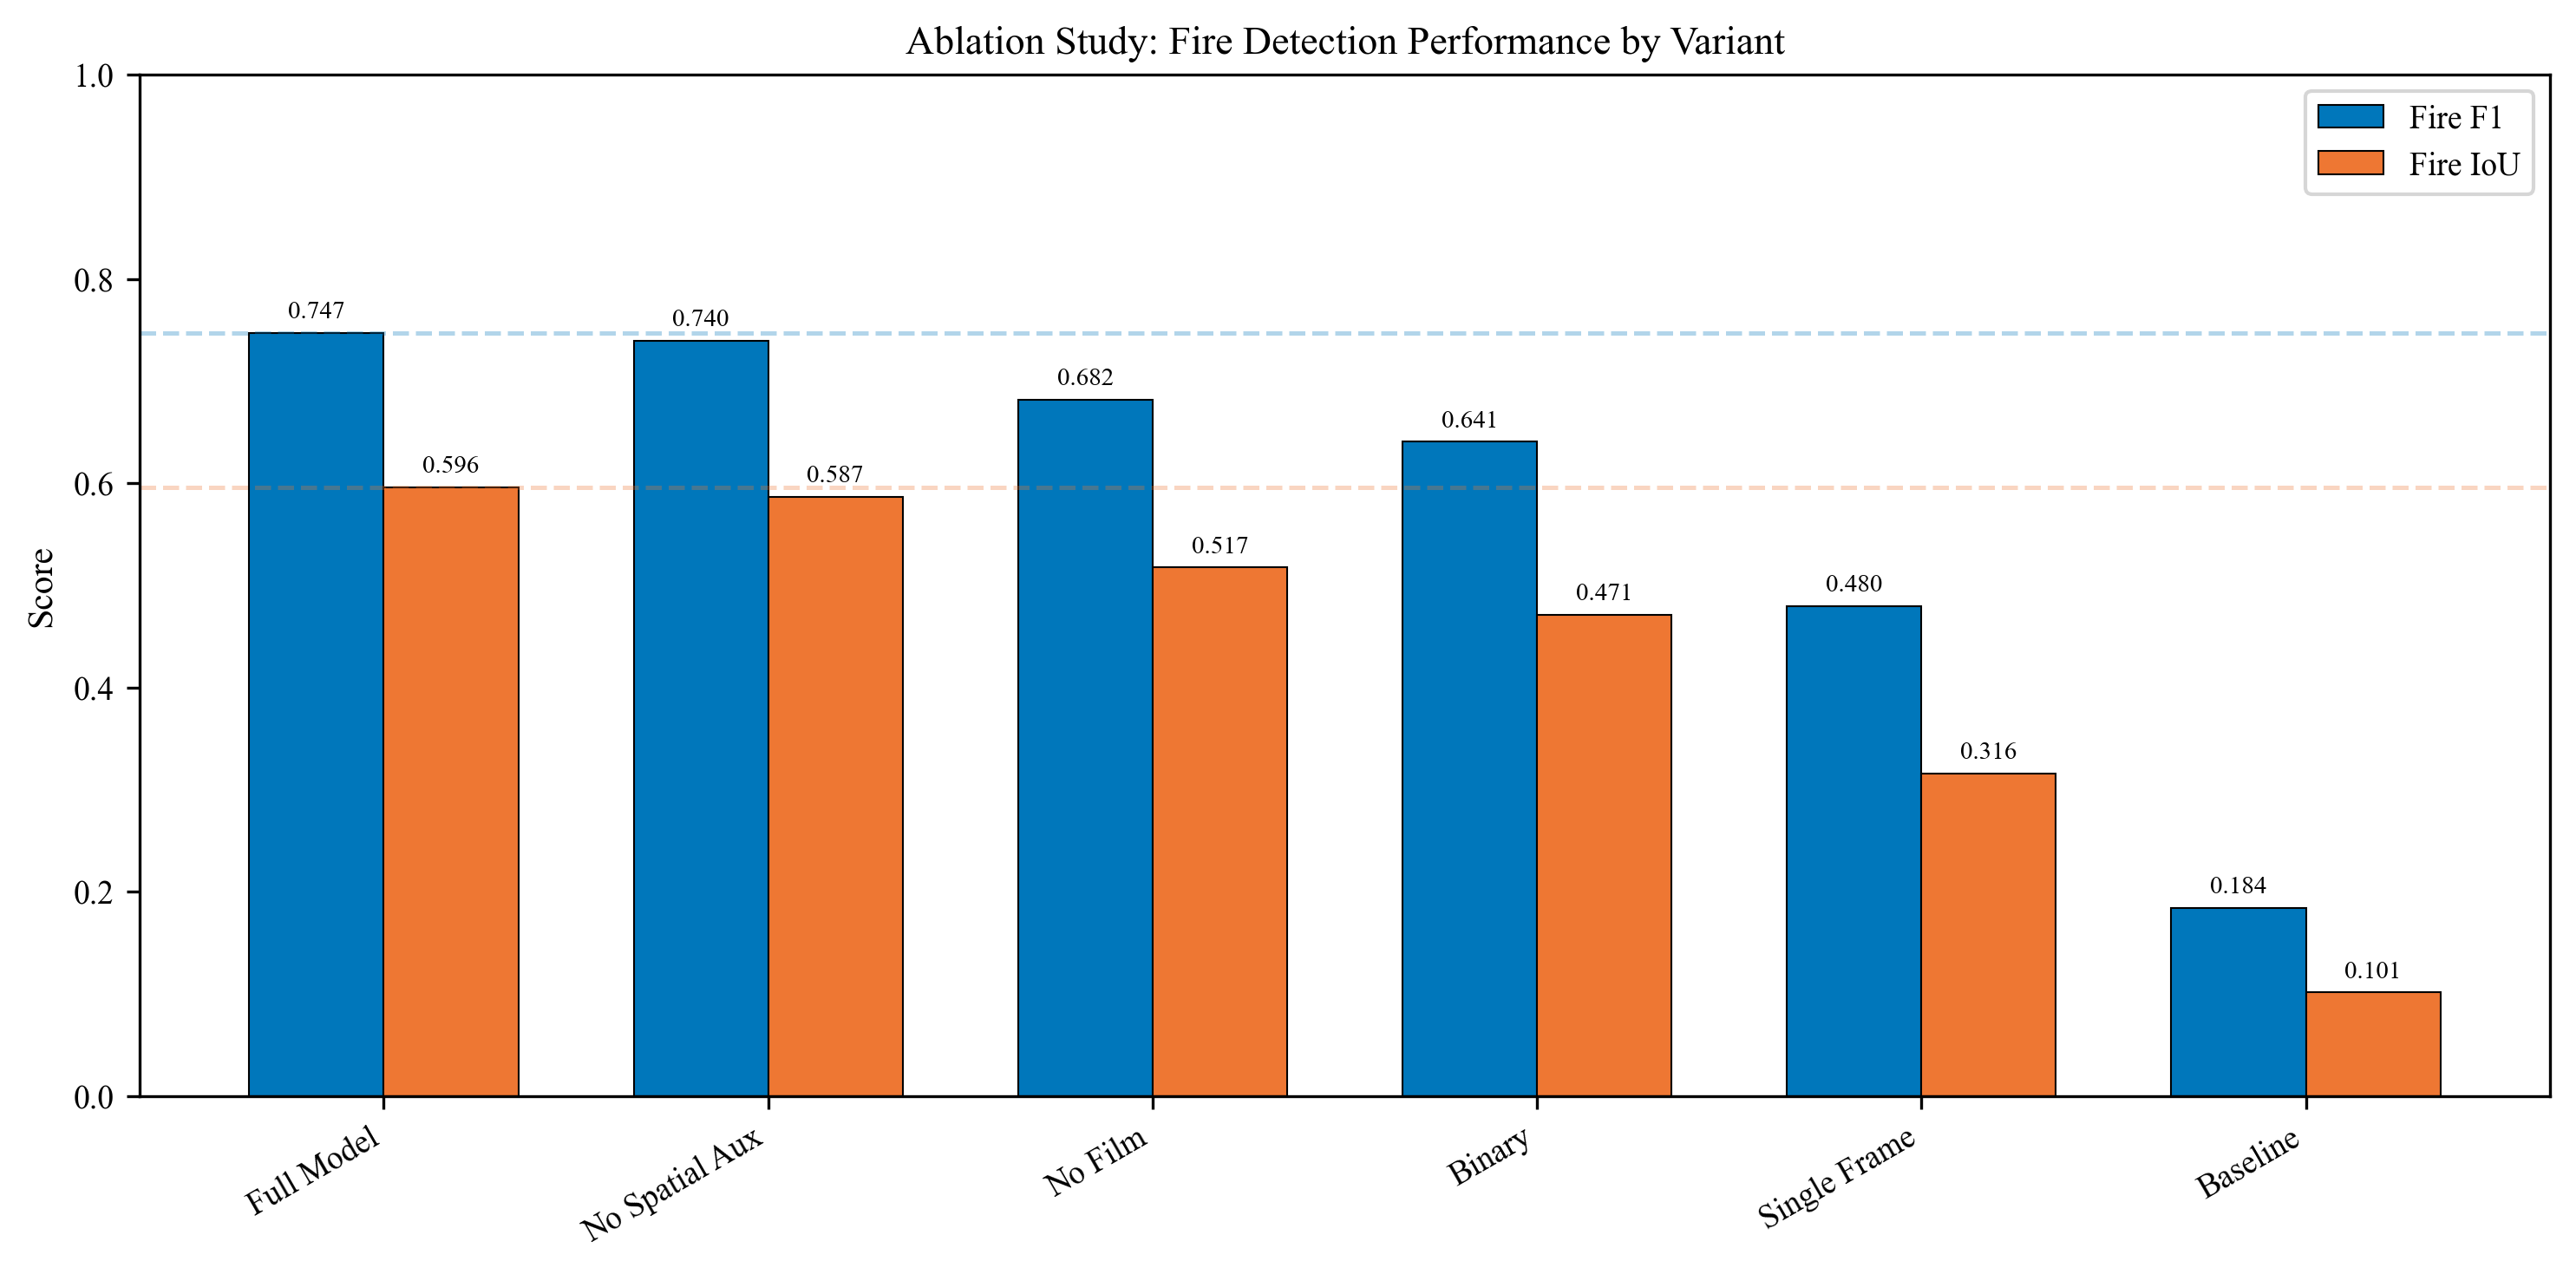
\includegraphics[width=\textwidth]{figures/fig6_ablation_results.png}
  \caption{Ablation study: fire detection performance by variant.}
  \label{fig:ablation}
\end{figure}


%% ======================================================================
\section{Discussion}
\label{sec:discussion}
%% ======================================================================

\subsection{Value of FiLM Weather Conditioning}

The ablation study reveals that FiLM conditioning primarily acts as a false-positive suppressor. Removing FiLM increases recall from 69.6\% to 84.0\% while decreasing precision from 80.6\% to 57.4\%, yielding a net fire F1 drop of 0.065. This indicates that weather context (drought indices, wind speed, humidity) helps the model distinguish genuinely burned areas from spectrally similar surfaces---bare soil, post-harvest agricultural stubble, and rocky outcrops---that appear fire-like under dry conditions but lack the meteorological precursors for actual fire events. The adaLN-Zero initialisation ensures stable integration during early training, while the learned modulation parameters specialise to suppress weather-inconsistent false positives.

\subsection{Severity Discrimination Limitations}

The inability to discriminate classes 2--4 stems from: (1) FRP-based label noise, (2) 82:11:4:2:1 class imbalance, and (3) 30~m spectral ambiguity for fine severity gradients. Future work should incorporate field-based CBI measurements and higher-resolution imagery.

\subsection{Training Foundation Models on Consumer Hardware}

LLRD-DP reduces VRAM from $\sim$24~GB to 3.7~GB by partitioning the backbone at a configurable depth boundary. This approach avoids LoRA's partial parameter freezing (incompatible with DirectML) while achieving comparable memory savings through explicit gradient graph partitioning.

\begin{figure}[htbp]
  \centering
  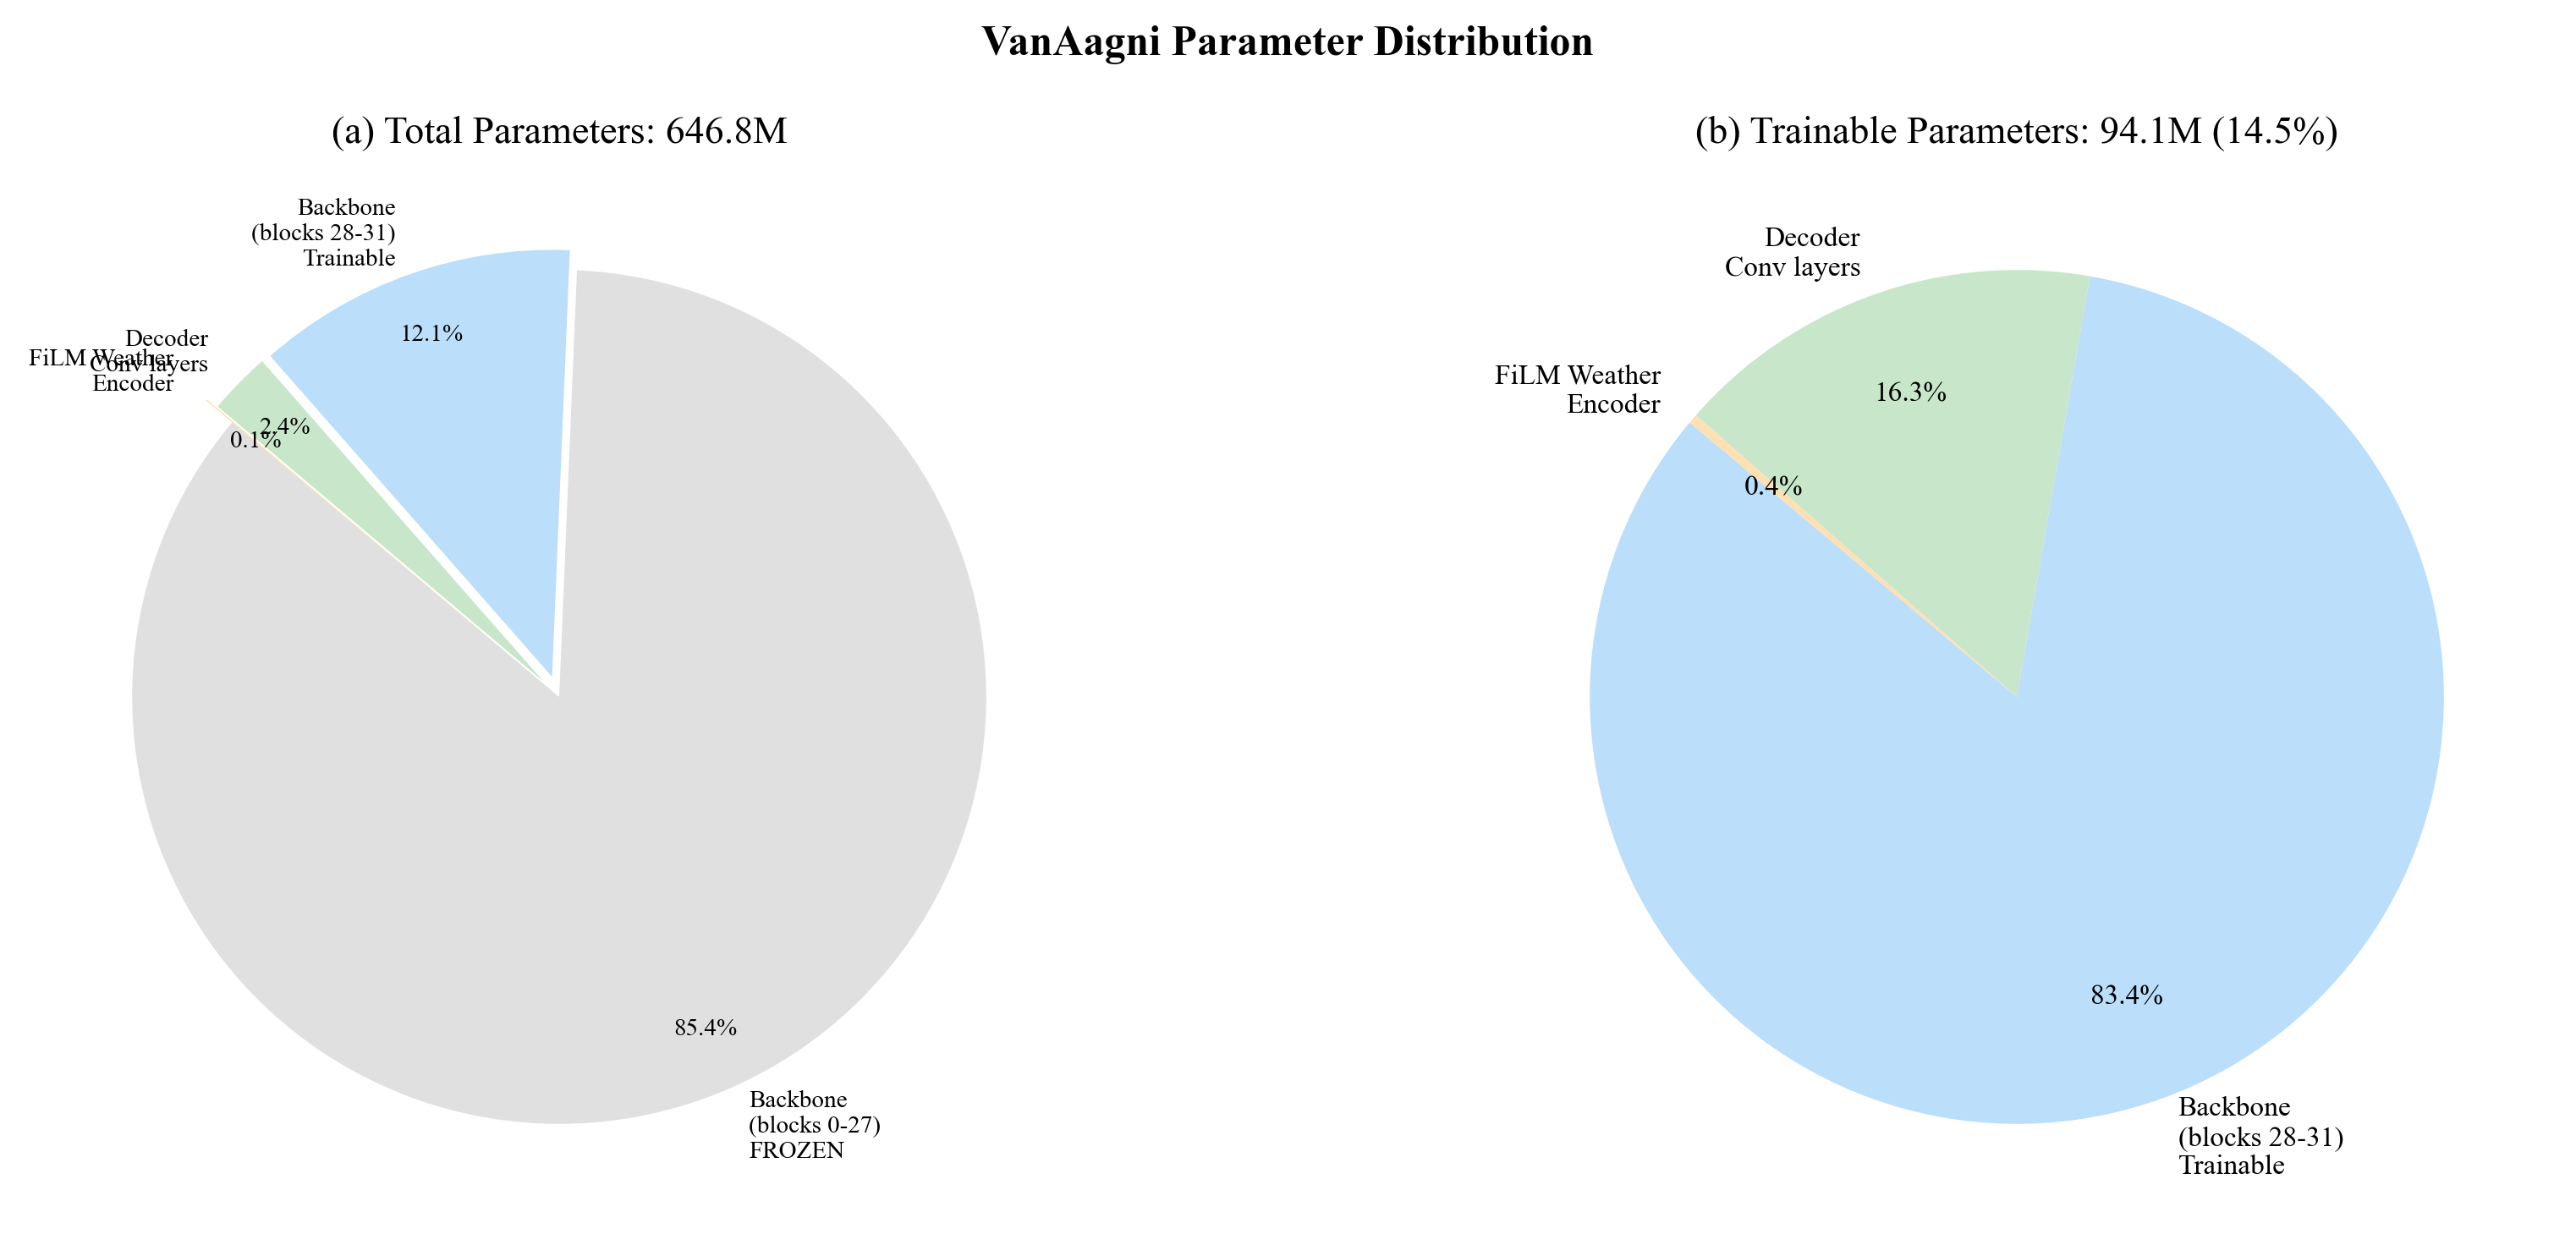
\includegraphics[width=0.8\textwidth]{figures/fig8_parameter_breakdown.png}
  \caption{Parameter distribution: 631M backbone (87.5\% frozen), 15.7M decoder, 0.3M FiLM.}
  \label{fig:params}
\end{figure}

\subsection{Operational Deployment}

VanAagni is deployed within the Van Suraksha Alert system serving 747 compartments across Guna Division, contributing burn severity maps to an integrated fire risk assessment that includes ignition probability (AUC = 0.9998) and intensity prediction.

\subsection{Limitations and Future Work}

Key limitations include geographic specificity, FRP-based label noise, and severity discrimination. Future directions include cross-biome transfer learning, multi-scale fusion with 10~m bands, and post-fire recovery trajectory analysis.


%% ======================================================================
\section{Conclusion}
\label{sec:conclusion}
%% ======================================================================

We presented VanAagni, a weather-conditioned foundation model architecture for 30-meter burn severity mapping. FiLM conditioning bridges spectral remote sensing and fire meteorology. Applied to 82 fire events in central India's Vindhyan forests, VanAagni achieves Fire F1 = 0.747 with 80.6\% precision and 69.6\% recall. The LLRD-DP strategy enables consumer GPU training (3.7~GB VRAM), demonstrating that foundation model research need not be constrained to datacenter environments. The tiered label quality system provides a framework for integrating heterogeneous fire reference data. VanAagni is deployed operationally within the Van Suraksha Alert system.


%% ======================================================================
\section*{Data and Code Availability}
%% ======================================================================

Model weights, training code, and ablation framework are available at [repository URL]. HLS S30: \url{https://lpdaac.usgs.gov/}. VIIRS: \url{https://firms.modaps.eosdis.nasa.gov/}. ERA5: \url{https://cds.climate.copernicus.eu/}. Prithvi-EO-2.0: \url{https://huggingface.co/ibm-nasa-geospatial/Prithvi-EO-2.0-600M-TL}.


%% ======================================================================
\section*{Acknowledgements}
%% ======================================================================

The author thanks the Madhya Pradesh Forest Department for operational support, NASA for Prithvi-EO-2.0 and HLS, and the TerraTorch team. Weather data: ERA5 (CCCS) and Open-Meteo. This work was conducted on a consumer AMD Radeon RX 9060 XT GPU via Microsoft DirectML.


%% ======================================================================
%% References
%% ======================================================================

\begin{thebibliography}{99}

\bibitem{giglio2018}
L. Giglio, L. Boschetti, D.P. Roy, M.L. Humber, C.O. Justice,
The Collection 6 MODIS burned area mapping algorithm and product,
\textit{Remote Sens. Environ.} 217 (2018) 72--85.

\bibitem{key2006}
C.H. Key, N.C. Benson,
Landscape assessment: ground measure of severity, the Composite Burn Index; and remote sensing of severity, the Normalized Burn Ratio,
in: \textit{FIREMON: Fire Effects Monitoring and Inventory System}, USDA Forest Service, RMRS-GTR-164-CD, 2006.

\bibitem{lentile2006}
L.B. Lentile, Z.A. Holden, A.M.S. Smith, M.J. Falkowski, A.T. Hudak, P. Morgan, S.A. Lewis, P.E. Gessler, N.C. Benson,
Remote sensing techniques to assess active fire characteristics and post-fire effects,
\textit{Int. J. Wildland Fire} 15 (2006) 319--345.

\bibitem{miller2007}
J.D. Miller, A.E. Thode,
Quantifying burn severity in a heterogeneous landscape with a relative version of the delta Normalized Burn Ratio,
\textit{Remote Sens. Environ.} 109 (2007) 66--80.

\bibitem{french2008}
N.H.F. French, E.S. Kasischke, R.J. Hall, K.A. Murphy, D.L. Verbyla, E.E. Hoy, J.L. Allen,
Using Landsat data to assess fire and burn severity in the North American boreal forest region,
\textit{Int. J. Wildland Fire} 17 (2008) 443--462.

\bibitem{parks2014}
S.A. Parks, G.K. Dillon, C. Miller,
A new metric for quantifying burn severity: the relativized burn ratio,
\textit{Remote Sensing} 6 (2014) 1827--1844.

\bibitem{roy2008}
D.P. Roy, L. Boschetti, C.O. Justice, J. Ju,
The collection 5 MODIS burned area product---Global evaluation by comparison with the MODIS active fire product,
\textit{Remote Sens. Environ.} 112 (2008) 3690--3707.

\bibitem{knopp2020}
L. Knopp, M. Wieland, M. Rättich, S. Martinis,
A deep learning approach for burned area segmentation with Sentinel-2 data,
\textit{Remote Sensing} 12 (2020) 2422.

\bibitem{hu2021}
X. Hu, Y. Ban, A. Nascetti,
A novel burned area detection approach using multi-temporal Sentinel-2 data,
\textit{Remote Sens. Environ.} 255 (2021) 112258.

\bibitem{seydi2022}
S.T. Seydi, V. Saeidi, B. Kalantar, N. Ueda, A.A. Halin,
Burnt-Net: Wildfire burned area mapping with single post-fire Sentinel-2 data and deep learning morphological neural network,
\textit{Ecol. Indic.} 140 (2022) 108999.

\bibitem{jakubik2024}
J. Jakubik, S. Chu, D. Phung, P. Bangalore, et al.,
Prithvi-EO-2.0: A versatile multi-temporal foundation model for Earth observation applications,
\textit{arXiv:2412.02981} (2024).

\bibitem{cong2022}
Y. Cong, S. Khanna, C. Meng, P. Liu, E. Rozi, Y. He, M. Burke, D. Lobell, S. Ermon,
SatMAE: Pre-training transformers for temporal and multi-spectral satellite imagery,
\textit{NeurIPS} (2022).

\bibitem{mendieta2023}
M. Mendieta, B. Han, X. Shi, Y. Zhu, C. Chen,
Towards geospatial foundation models via continual pretraining,
\textit{IEEE ICCV} (2023) 16806--16816.

\bibitem{hu2022lora}
E.J. Hu, Y. Shen, P. Wallis, Z. Allen-Zhu, Y. Li, S. Wang, L. Wang, W. Chen,
LoRA: Low-rank adaptation of large language models,
\textit{ICLR} (2022).

\bibitem{perez2018}
E. Perez, F. Strub, H. de Vries, V. Dumoulin, A. Courville,
FiLM: Visual reasoning with a general conditioning layer,
\textit{AAAI} 32 (2018).

\bibitem{peebles2023}
W. Peebles, S. Xie,
Scalable diffusion models with transformers,
\textit{IEEE ICCV} (2023) 4195--4205.

\bibitem{vanwagner1987}
C.E. Van Wagner,
\textit{Development and Structure of the Canadian Forest Fire Weather Index System},
Forestry Technical Report 35, Canadian Forestry Service, Ottawa, 1987.

\bibitem{flannigan2005}
M.D. Flannigan, K.A. Logan, B.D. Amiro, W.R. Skinner, B.J. Stocks,
Future area burned in Canada,
\textit{Clim. Change} 72 (2005) 1--16.

\bibitem{fsi2023}
FSI,
\textit{India State of Forest Report 2023},
Forest Survey of India, Dehradun, 2023.

\bibitem{claverie2018}
M. Claverie, J. Ju, J.G. Masek, J.L. Dungan, E.F. Vermote, J.C. Roger, S.V. Skakun, C. Justice,
The Harmonized Landsat and Sentinel-2 surface reflectance data set,
\textit{Remote Sens. Environ.} 219 (2018) 145--161.

\bibitem{collins2018}
L. Collins, P. Griffioen, G. Newell, A. Mellor,
The utility of Random Forests for wildfire severity mapping,
\textit{Remote Sens. Environ.} 216 (2018) 374--384.

\bibitem{hislop2019}
S. Hislop, S. Jones, M. Soto-Berelov, A. Skidmore, A. Haywood, T.H. Nguyen,
A fusion approach to forest disturbance mapping using time series ensemble techniques,
\textit{Remote Sens. Environ.} 221 (2019) 188--197.

\bibitem{ronneberger2015}
O. Ronneberger, P. Fischer, T. Brox,
U-Net: Convolutional networks for biomedical image segmentation,
\textit{MICCAI} (2015) 234--241.

\bibitem{lin2017focal}
T.-Y. Lin, P. Goyal, R. Girshick, K. He, P. Dollar,
Focal loss for dense object detection,
\textit{IEEE ICCV} (2017) 2980--2988.

\bibitem{sudre2017}
C.H. Sudre, W. Li, T. Vercauteren, S. Ourselin, M.J. Cardoso,
Generalised dice overlap as a deep learning loss function for highly unbalanced segmentations,
\textit{DLMIA/ML-CDS} (2017) 240--248.

\bibitem{loshchilov2019}
I. Loshchilov, F. Hutter,
Decoupled weight decay regularization,
\textit{ICLR} (2019).

\bibitem{farr2007}
T.G. Farr, P.A. Rosen, E. Caro, et al.,
The Shuttle Radar Topography Mission,
\textit{Rev. Geophys.} 45 (2007) RG2004.

\bibitem{zanaga2022}
D. Zanaga, R. Van De Kerchove, D. Daems, et al.,
ESA WorldCover 10 m 2021 v200,
\textit{Zenodo} (2022).

\bibitem{hersbach2020}
H. Hersbach, B. Bell, P. Berrisford, et al.,
The ERA5 global reanalysis,
\textit{Q. J. R. Meteorol. Soc.} 146 (2020) 1999--2049.

\bibitem{bernstein2024}
J. Bernstein, P. Bangalore, et al.,
TerraTorch: A library for geospatial foundation model fine-tuning,
\textit{arXiv preprint} (2024).

\end{thebibliography}

\end{document}
